% !TeX root = skripta-konstitutivni-vztahy.tex
% !TeX lastmodified = 2006-09-11

\subsection{Co je to elasticita?}
Elasticita je schopnost látky vrátit se po zatížení a~odlehčení do původního tvaru.
Podle tvaru deformačně-napěťové charakteristiky dělíme tyto látky na lineárně a~nelineárně elastické.

Charakteristiky:
\begin{figure}[H]
	\label{fig:linearne-elasticka-latka}
	\centering
	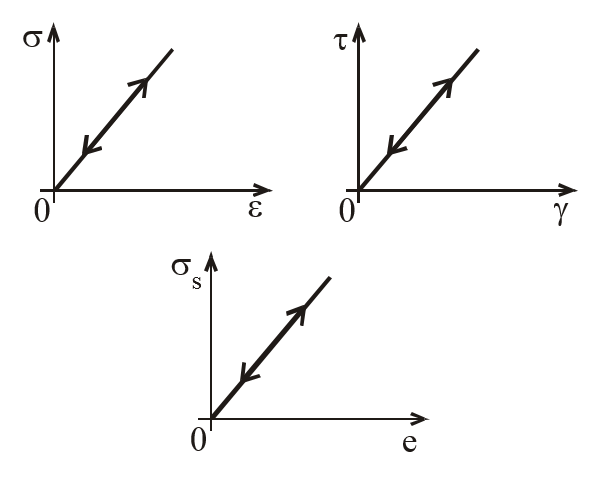
\includegraphics[width=0.7\linewidth]{linearne-elasticka-latka}
	\caption{lineárně elastické látky}
\end{figure}

\begin{figure}[H]
	\label{fig:nelinearne-elasticka-latka}
	\centering
	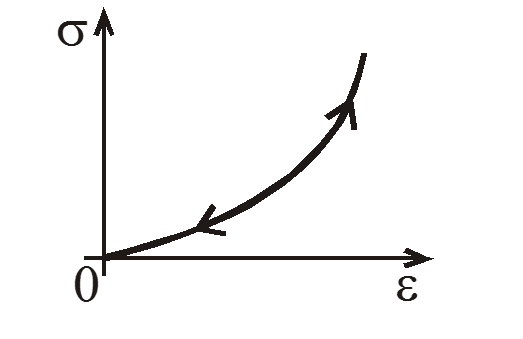
\includegraphics[width=0.7\linewidth]{nelinearne-elasticka-latka}
	\caption{nelineárně elastické látky}
\end{figure}
